\chapter{Winding-Flux Clipping Audit}
\label{app:clipping}

This appendix documents the audit underlying the
$|W| \le 10^{8}$ guard introduced in \S\ref{sec:data-clip} and
recorded as Finding~F2.

\section{Physical range}
\label{app:clip-phys}

The per-pixel magnitude of the magnetic winding flux $W$ in the
present corpus is approximately bounded by
$|W| \sim 10^{7}$ across the twenty-one cubes after quality
filtering. The peak values reflect localised current-carrying
structures in emerging flux tubes and are physically
load-bearing; clipping them at $10^{5}$, as in an earlier
revision of the pipeline, removed the signal in the
$10^{5}$--$10^{7}$ dynamic range that the encoder is required to
represent.

The single exception in the corpus is \texttt{harp\_8}, which
contains a small population of pixels whose values exceed
$10^{10}$ in absolute value. These pixels are localised to a
spatial cluster within the cube and are consistent with a
known photospheric-measurement pathology rather than physical
winding flux. A guard of $|W| \le 10^{8}$ ($10\times$ above the
nominal physical peak) preserves the signal in the remaining
twenty cubes while clipping the \texttt{harp\_8} pathology.

\section{Histogram and per-cube outlier counts}
\label{app:clip-fig}

\begin{figure}[htbp]
\centering
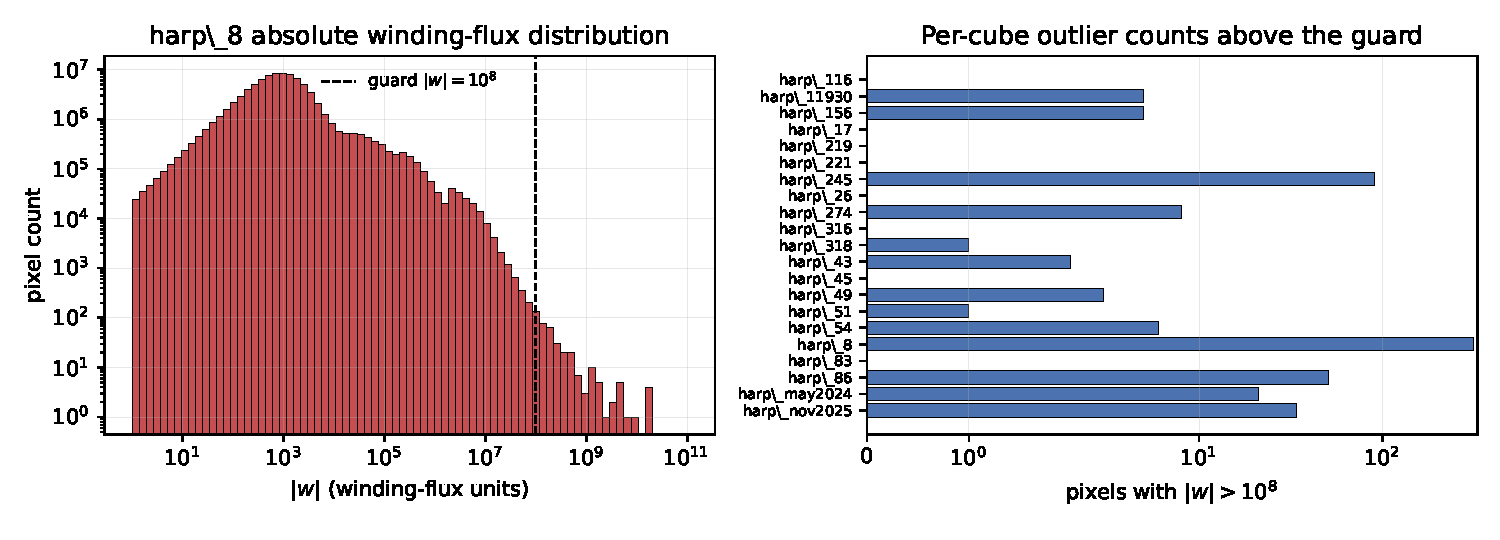
\includegraphics[width=0.97\linewidth]{assets/figures/clip_audit.pdf}
\caption{Left: log--log histogram of $|W|$ values across the
\texttt{harp\_8} cube, with the $10^{8}$ guard marked. The
pathology forms a thin tail extending to
$\approx 10^{10}$, well separated from the physical bulk.
Right: per-cube count of pixels exceeding the guard, on a
symmetric-log axis. All twenty cubes other than \texttt{harp\_8}
contribute zero or single-digit pixel counts; \texttt{harp\_8}
contributes the majority of all clipped pixels in the corpus.}
\label{fig:clip-audit}
\end{figure}

\section{Guard implementation}
\label{app:clip-impl}

The guard is implemented in
\texttt{solarflare\_data/zarr\_loader.py} as a clip operation on
the lazy zarr read path, before downstream consumers (the
sampler and the encoder) observe the data. The clip is
sign-preserving: $W' = \mathrm{clip}(W,\, -10^{8},\, +10^{8})$.
The corresponding constant in the code base is
\texttt{WIND\_FLUX\_CLIP = 1e8}; the older constant
\texttt{BZ\_CLIP\_GAUSS = 1e5}, which destroyed signal, is no
longer present.

A spatial-clustering investigation of the \texttt{harp\_8}
outliers, motivated by the possibility that the pathology
represents a recoverable instrument artefact rather than
unrecoverable noise, is deferred to future work
(Chapter~\ref{ch:summary}).
